\section{Use cases and User Guide}
In this section we come to some use cases of the FracTime animations, the user gameplay and instruction of MagicVR.

TODO! pictures\\
\begin{figure}[!ht]
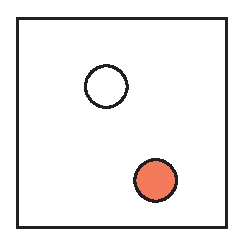
\includegraphics[width=0.4\textwidth]{pictures/sample.eps}
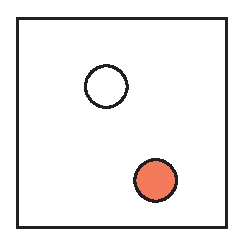
\includegraphics[width=0.4\textwidth]{pictures/sample.eps}
\caption{Scene Overview}
\end{figure}

\subsection{Element Stones}
In the virtual scene are placed some columns with \lq\lq{}Elementary Stones\rq\rq{}. They have different symbols as texture representing the according element and at the same time the 3D-Gesture which has to be performed to call this element. Those \lq\lq{}Elementary Stones\rq\rq{} can also be used to practice and get used to the 3D-Gestures.

If the a 3D-Gestures of one of the elements is correctly recognized, a BubbleAnimation as explained before starts to run, letting the user know, which element he activated.

\subsection{Shooting Elements}
If practiced enough, the user can feel free to move on to shoot elements. This is done by a combination of 3D-Gestures:
\begin{itemize}
\item{1.} Make a circle gesture: This activates the \lq\lq{}Shoot Mode\rq\rq{}. You will see this as there should appear a neutral ball at the top of your wand.
\item{2.} Make the element gesture of your wish: This calls the element. You should see that the ball at the top of your wand changes into the according element - equal to the element bubbles you saw on the elementary stones.
\item{3.} Make a multiplication gesture: This allows later on to shoot multiple element bubbles at once according to how many times you use this gesture. You should notice, that the ball at the top of the wand grows according to the multiplication.
\item{4.} Shoot the element using the shoot gesture. The element bubbles will shoot out of your wand searching its way to the according interaction. If you had multiplication done, you will see the ball shrink while shooting multiple bubbles.
\end{itemize}

\subsubsection{Fire and Water}
TODO! pictures\\
\begin{figure}[!ht]
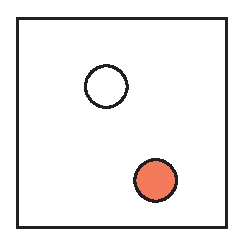
\includegraphics[width=0.4\textwidth]{pictures/sample.eps}
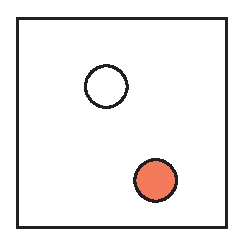
\includegraphics[width=0.4\textwidth]{pictures/sample.eps}
\caption{Fire and Water gestures}
\end{figure}

Element bubbles of the type water and fire will have their target on the fireplace located at the left side of the scene. Fire bubbles make the fire grow bigger while water will shrink it down.

\subsubsection{Lightning}
TODO! picture\\
\begin{figure}[!ht]
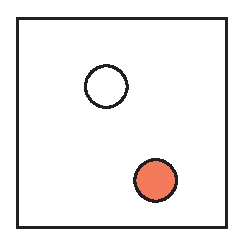
\includegraphics[width=0.4\textwidth]{pictures/sample.eps}
\caption{Lightning gesture}
\end{figure}

Element bubbles of the type Lightning will have their target at the lantern placed in the front part of the scene. As it is hit by the bubbles, the scene will be lit more and more.

\subsubsection{Wind}
TODO! picture\\
\begin{figure}[!ht]
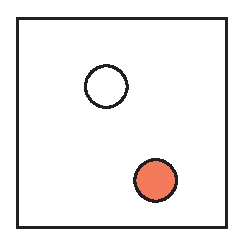
\includegraphics[width=0.4\textwidth]{pictures/sample.eps}
\caption{Wind gesture}
\end{figure}
TODO! description\\